\documentclass[../ana1.tex]{subfiles}
\onlyinsubfile{\sectionNumbering} %Use numbering relative to sections and not subsection

\begin{document}
\setcounter{section}{8}

\section{Cauchyfolgen}
\begin{defi}[Cauchyfolge]
	Eine Folge \({(a_n)}_n\) heißt Cauchyfolge (kurz Cauchy), falls
	\[\forall \varepsilon > 0 \,\exists K\in\N: |a_n-a_m| < \varepsilon \, \forall n,m\geq K \]
\end{defi}
\begin{bem}
	Reicht \(m,n\in\N \) mit \( m>n\geq K \) zu betrachten, da Def.\ symmetrisch in \(m,n\) ist und falls \(m=n \Rightarrow a_m-a_n=0\)
\end{bem}
\begin{lem}
	Jede konvergente Folge ist eine Cauchyfolge.
\end{lem}
\begin{bew}
	\( {(a_n)}_n \quad a_n \rightarrow a \) für \(n\rightarrow\infty \) \\
	d.\ h.\  \( \forall \varepsilon > 0 \exists K \in \N: \forall n\geq K \) ist \( |a_n-a| < \varepsilon/2 \).\\
	Ist \(m>n\geq K: |a_m -a_n| = |a_m-a+a-a_n| \leq \underbrace{|a_m-a|}_{<\varepsilon/2} + \underbrace{ |a-a_n| }_{<\varepsilon/2}. \) Also ist \({(a_n)}_n\) Cauchyfolge.
\end{bew}
\begin{lem}
	Jede Cauchyfolge ist beschränkt.
\end{lem}
\begin{bew}
	Sei \(a_n\) Cauchyfolge. 
	\[ \forall \varepsilon > 0 \, \exists K\in\N:|a_m-a_n| < \varepsilon \quad \forall m,n\geq K. \]
	Wähle \(\varepsilon = 1, k_0: |a_m-a_n| < 1 \quad \forall n,m\geq K_0 \) \\
	Sei \(n \geq k_0 \Rightarrow |a_{K_0} - a_n| < 1. \)
	\[ \Rightarrow |a_n| = |a_n - a_{K_0} + a_{K_0}| \leq |a_n - a_{K_0}| + |a_{K_0}| < 1 + |a_{K_0}| \] für alle \(n\geq K_0\) \\
	Also setze: \( C := \max ( |a_1|,|a_2|,\ldots,|a_{K_0}|,1+|a_{K_0}| ) < \infty \) 
	\[ \Rightarrow \forall n\in\N \text{ ist } |a_n| \leq C. \]
\end{bew}
\begin{bsp}
	\begin{align*}
		a_n = {(-1)}^n \text{ (oder } (-1)^n + 1/n \text{)} \\
		n = 2k, k\in\N \Rightarrow a_{2k} = {(-1)}^{2k} = 1 \\
		a_{2k+1} = {(-1)}^{2k+1} = -1.
	\end{align*}
	Die neue Folge \( {(a_{2k})}_{k\in\N} \) ist konstant, also konvergiert sie.
\end{bsp}
\begin{bsp}
	\(B= \{b_1, b_2,\ldots,b_R \} \subset \R \quad R\in\N \).\\
	\( {(a_n)}_n \) Folge mit Werten in \(B\).
	\(a_n \in B \, \forall n\in\N \) \\
	\(B\) endliche Menge!\\
	\( \Rightarrow \) Es gibt mindestens ein \(r_0 \in \{1,2,\ldots,R\} \), sodass \( a_n=b_{r_0}  \) für unendlich viele \(n\).\\
	\[ \Leftrightarrow \forall K\in\N \,\exists n>K : a_n = b_{r_0} \]
	Jetzt induktiv: \\
	\begin{align*}
		n_1 \in\N: a_{n_1} = b_{r_0}.\\
		n_2 := \min (n>n_1:a_n=b_{r_0}) >n_1 \quad a_{n_2} = b_{r_0}\\
		\text{induktiv}\\
		\text{geg. } n_1 < n_2<\cdots<n_k\\
		a_{n_l} = b_{r_0} \quad l = \{1, \ldots,k \} \\
		n_{k+1} = \min(n>n_k:a_n = b_{r_0}) > n_k \text{ und } a_{n_{k+1}} = b_{r_0}.
	\end{align*}
	Erhalte \(n_k\in\N \quad \forall n\in\N \) mit \( n_{k+1} > n_k \forall k\in\N \) und \( a_{n_k} = b_{r_0} \) \\
	\( \Rightarrow \) Folge \( {(a_{n_k})}_{k\in\N} \) die konstant ist.\\
	Außerdem \( {(a_{n_k})}_k \) ist Teil der Folge \( {(a_n)}_n \)!
\end{bsp}
\begin{defi}[Teilfolge]
	Eine Funktion \( \sigma:\N \rightarrow\N \) heißt Ausdünnung, falls \( \sigma (n+1) > \sigma(n) \quad \forall n\in\N \) (d.\ h.\  \(\sigma \) ist streng monoton wachsend).
\end{defi}
Erinnerung: Folge ist eine Funktion \(f: \N\rightarrow X \) \\
\( \sigma : \N\rightarrow\N \Rightarrow f \circ \sigma : \N\rightarrow X, n\mapsto f(\sigma(n))  \) ist auch eine Folge.\\
\(a_n = f(n),\qquad a_{\sigma(n)} = f(\sigma(n)) = (f\circ\sigma)(n) \) \\
Geg. Folge \( {(a_n)}_{n\in\N} \) und eine Ausdünnung \( \sigma : \N\rightarrow \N. \) Setzen wir \( n_k := \sigma (k), k\in\N \) und \( {(a_{\sigma(k)})}_k = {(a_{n_k})}_{k\in\N} \) Teilfolge von \( {(a_n)}_{n\in\N} \).\\
Beobachtung: abgeschlossene und beschränkte Intervalle sind aus Folgensicht fast so gut wie endliche Mengen!
\begin{lem}
	Sei \(I = [b,c], \quad b,c\in\R, b\leq c.\ {(a_n)}_n \subset I \). \Dphp{} \(a_n \in I \quad\forall n\in\N \), dann gibt es eine Teilfolge, von \({(a_n)}_n\), die mit Grenzwert in \(I\) konvergiert.
\end{lem}
\begin{bew}
	\(I_0 = [a,b]\) \\
	Bild:\\
	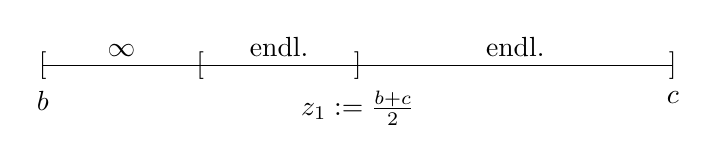
\begin{tikzpicture}[scale = 8]
		\draw (0,0) -- (1,0);
		\draw (0,0) node {\([\)} node[below = 2mm] {\(b\)};
		\draw (1,0) node {\(]\)} node[below = 2mm] {\(c\)};
		\draw (1/2,0) node {\(]\)} node[below = 2mm] {\(z_1:=\frac{b+c}{2}\)};
		\draw (1/4,0) node {\([\)};
		\draw (3/4,0) node[above] {endl.};
		\draw (3/8,0) node[above] {endl.};
		\draw (1/8,0) node[above] {\(\infty\)};
	\end{tikzpicture}
	\\
	%29.11.2018
	Fallunterscheidung:\\
	1.) Es sind \(\infty \)-viele \( a_n\in I_1 := [b,z_1] \). Dann setze \(b_1 := b, c_1 := z_1, I_1 = I_{1,-} = [b_1,c]\).\\
	2.) Nun endlich viele \(a_n\in I_{1,-} \Rightarrow b_1 := z_1, c_1 := c, I_1 := I_1 := I_{1,+} := [z_1,c] = [b_1,c_1] \Rightarrow \exists \infty \)-viele \(a_n \in I_1\).\\
	\(|I_1| = \) Länge von \(I_1 = c_1-b_1 = \frac{c-b}{2} \). \(n_1 = \min (n\in\N:a_n \in I_1)  \Rightarrow n_1 \geq 1. a_{n_1} \in I_1 \).
	Dann \(z_2 := \frac{b_1 + c_1}{2}\) \\
	\(\Rightarrow \) Sind \(\infty \)-viele \(a_n\in I_{2,-} := [b_1,z_2] \), so setze \(I_2 := I_{2,-}\). Somit sind \(\infty \)-viele \(a_n\in I_{2,+} = [z_1,c_1] \). Setze dann \(I_2 := I_{2,+}\).\\
	\[ n_2 := \min(n>n_1:a_n\in I_2) \Rightarrow a_{n_2} \in I_2 \text{ und } n_2>n_1\geq 1. |I_2| = \frac{|I_1|}{2} = \frac{c-b}{2}. \]
	Iteriere dies: Ang.\ haben \(I_k = [b_k, c_k] \subset I_{k-1} \subset \ldots \subset I_1 \subset I_0 = [b,c]. |I_k| = \frac{|I_0|}{2^k}. \) \\
	\(z_{k+1} := \frac{b_k + c_k}{2} \) Mittelpunkt von \(I_k\).\\
	Sind \(\infty \)-viele \(a_n\) in \(I_{k+1} := [b_k, z_{k+1}] \), so setze \(I_{k+1} := I_{k+1,-} \qquad b_{k+1} = b_k, c_{k+1} = z_k+1 \).\\
	Somit \(I_{k+1} := I_{k+1,+} = [z_{k+1, c_k}]/ b_{k+1} = z_{k+1}, c_{k+1} = c_k. \) \\
	Nach Konstruktion sind \(\infty \)-viele \(a_n\in I_{k+1} \). (d.\ h.\  \(\forall K\in\N \exists n>k:a_n\in I_{k+1} \))\\
	\( n_{k+1} := \min (n>n_k: a_n \in I_{k+1}) > n_k\\
	\Rightarrow \) Folge von Indizes \(n_1 <n_2<\cdots<n_k<n_{k+1}<\ldots \\
	n_k\in\N \) mit \( a_{n_k} \in I_k, |I_k| = \frac{|I_0|}{2^k}\\
	I_k = [b_k, c_k] \)
	\[b_k \leq a_{n_k} \leq c_k \quad \forall k\in\N (*) \]
	\( {(b_k)}_k \) monoton wachsende Folge \(b_k\leq c \forall k \).\\
	\( {(c_k)}_k \) monoton fallende Folge \( c_k \geq b \forall k \).\\
	\( \overset{\text{Mon. Konv.}}{\Rightarrow} \\b= \limes{k} b_k \) exist.\\
	\(c = \limes{k} c_k \) exist.\\
	und \(0 \leq c_k - b_k \leq \frac{c-b}{2^k} \rightarrow0 (k\rightarrow\infty) \).\\
	\(\Rightarrow b=c \overset{(*)}{\Rightarrow} {(a_{n_k})}_k \) konvergiert gegen \(b\).\\
	d.\ h.\  \( {(a_{n_k})}_k \) ist konv.\ Teifolge von \( {(a_n)}_n \).
	%Der unendliche Intervall wird immer halbiert in einen endlichen und unendlichen Teil (rekursiv).
\end{bew}
\begin{kor}
	Jede beschränkte (reelle) Folge hat eine konvergente Teilfolge (Satz von Bolzano-Weierstraß).
\end{kor}
\begin{bew}
	Sei \( 0\leq C < \infty. |a_n| \leq C \quad\forall n\in\N. \) \\
	\[ \Rightarrow -C \leq a_n \leq C, a_n \in [-C, C] \quad\forall n\in\N. \]
	\( \Rightarrow \) Beh.\ folgt aus Lemma 5!
\end{bew}
\begin{kor}
	Jede Cauchy-Folge hat eine konv. Teilfolge.
\end{kor}
\begin{bew}
	Nach Lemma 3 ist \( {(a_n)}_n \) beschränkt. Wende Korrolar 6 an.
\end{bew}
Hauptbeobachtung:
\begin{lem}
	Sei \({(a_n)}_n\) eine Cauchyfolge. Dann gilt
	\[ {(a_n)}_n \text{ konvergiert } \Leftrightarrow {(a_n)}_n \text{ hat eine konvergente Teilfolge.} \]
\end{lem}
\begin{bem}
	Ist \( {(a_n)}_n \) konvergente Folge, so konvergiert jede Teilfolge gegen den gleichen Grenzwert von \({(a_n)}_n\).
\end{bem}
\begin{bem}
	\( {(a_n)}_n \) Cauchyfolge \\
	\begin{align*}
		&\Leftrightarrow \forall \varepsilon>0 \,\exists K\in\N:|a_m-a_n|<\varepsilon \quad \forall m>n\geq K.\\
		&\Leftrightarrow \forall \varepsilon>0 \,\exists K\in\N:|a_{n+p}-a_n|<\varepsilon \quad \forall n\geq K, p\in\N \\
		&\Leftrightarrow \forall \varepsilon>0 \,\exists K\in\N:\sup \underbrace{\set{|a_{n+p}-a_n|}}_{\substack{\text{muss gleichm.}\\\text{in }p\in\N\text{ klein sein}\\ \text{für } n \text{ groß} }}<\varepsilon \quad \forall n\geq K, p\in\N.
	\end{align*}
\end{bem}
\begin{bew}
	\glqq{}\( \Rightarrow \)\grqq{}: Nach Bem 1 konvergiert jede Teilfolge von \( {(a_n)}_n \) gegen denselben Grenzwert.\\
	\glqq{}\(\Leftarrow \)\grqq{}: Ang. Teilfolge \( {(a_{n_k})}_k \) konvergiert gegen \(L\in\R \). \(L = \limes{k} a_{n_k} \) existiert.\\
	\( n_k\in\N, n_1<n_2<\cdots<n_k<n_{k+1}<\ldots \) \\
	Auch: \({(a_n)}_n\) ist Cauchy, d.\ h.\ 
	\[ \forall \varepsilon>0\exists K\in\N:|a_m-a_n|<\varepsilon \quad\forall m>n\geq K (*). \]
	\[n_1 \geq 1 \Rightarrow n_2 > n_1 \geq 1 \Rightarrow n_2 \geq 2 \ldots n_k \geq k \forall k \]
	D.\ h.\ ist \(k>n \Rightarrow m=n_k \geq k>n \overset{(*)}{\Rightarrow} |a_{n_k}-a_n|<\varepsilon \quad \forall k>n\geq K \).\\
	Sei \( \varepsilon>0, K\) gegeben\\
	\[ \Rightarrow |a_{n_k} - a_n| <\varepsilon \quad \forall k>n\geq K \Rightarrow \limes{k} |a_{n_k}-a_n| = \limes{k} |a_{\sigma(k)}-a_n| = |L-a_n| \leq \varepsilon \]
	\(\sigma(k) = n_k, \limes{k} a_{\sigma(k)} = L \)
	\[ \forall \varepsilon>0 \exists K\in\N: |L-a_n|\leq \varepsilon \forall n\geq K \]
	\(\Rightarrow {(a_n)}_n\) konvergiert gegen \(L\)!
\end{bew}
\begin{satz}
	Eine (reelle) Folge \({(a_n)}_n\) konvergiert \( \Leftrightarrow {(a_n)}_n \) ist Cauchyfolge.
\end{satz}
\begin{bew}
	\glqq{}\(\Rightarrow \)\grqq{} ist Lemma 2.\\
	\glqq{}\( \Leftarrow \)\grqq{} \({(a_n)}_n\) Cauchy \( \overset{\text{Kor. 7}}{\Rightarrow} \exists \) konv. Teilfolge von \({(a_n)}_n \overset{\text{Lem. 8}}{\Rightarrow} {(a_n)}_n \) konvergiert. 
\end{bew}
z. B. \({(a_n)}_n\) Cauchyfolge. \(\Rightarrow \exists \) Teilfolge mit \(|a_{n_{k+1}}-a_{n_k}| <2^{-k}\).

\end{document}